\documentclass{article}
\usepackage{fixltx2e}
\usepackage[utf8]{inputenc}
\usepackage{graphicx}
\usepackage{sidecap}
\usepackage{fancyhdr}
\usepackage[margin=1.5in]{geometry}
\usepackage{amssymb,amsmath}
\usepackage[euler]{textgreek}
\usepackage[swedish]{babel}
\usepackage[framed,numbered,autolinebreaks]{mcode}


\setlength{\headheight}{21pt}

\begin{document}

% Titelsida -----------------------------
\begin{titlepage}
\begin{center}

% Upper part of the page. The '~' is needed because \\
% only works if a paragraph has started.

~\\
~\\
\textsc{\LARGE Link{\"o}pings Universitet}\\[1.5cm]


% Title
~\\
~\\
{ \huge \bfseries Modellbaserad reglering av dubbeltankar \\[0.4cm] }

% Author and supervisor
\large
\emph{Av:}\\
Hans-Filip \textsc{Elo} och Niklas \textsc{Ericson}

\vfill

% Bottom of the page
{\large \today}

\end{center}

% Slut på titelsida. ---------------------

% Innehåll ------------------------------
\newpage
\thispagestyle{empty}
\tableofcontents
~\\

\begin{center}
\line(1,0){400}
\end{center}

\listoffigures
~\\

\begin{center}
\line(1,0){400}
\end{center}

\listoftables

\end{titlepage}
%header ---------------------------------
\pagestyle{fancy}

\fancyhead{} % clear all header fields
\fancyhead[L]{TSRT12\slshape}
\fancyhead[R]{\today \slshape}

\fancyfoot{} % clear all footer fields
\fancyfoot[L,R]{\thepage}
\fancyfoot[L]{Modellbaserad reglering av dubbeltankar}

%slut på header ---------------------------------


\section{Inledning}
En överföringsfunktions egenskaper så som stigtid, översläng och felmarginal går att påverka genom att multiplicera funktionen med en deriverande, F\textsubscript{lead}, och en integrerande, F\textsubscript{lag}, funktion. En laboration med ett dubbeltanksystem har genomförts för att applicera teorin i verkligheten.


% ------------- Syfte -----------------------


\section{Syfte}
Syftet med laborationen var att färdigställa en överföringsfunktion för systemet med dubbeltankar och sedan reglera systemet så det uppnår givna specifikationskrav kring den givna arbetspunkten 10 cm vattennivå. 


% ------------- Metod -----------------------


\section{Metod}

En överföringsfunktion för systemet var given enligt nedan. 

\begin{equation}
G\textsubscript{dubbel}(s) = \frac{K_{enkel1}}{sT+1} * \frac{K_{enkel2}}{sT+1} = \frac{K\textsubscript{dubbel}}{(sT+1)^2}
\end{equation}
\\
Där {\itshape T}, K\textsubscript{enkel1} och K\textsubscript{enkel2} är konstanter. K\textsubscript{dubbel} är produkten av K\textsubscript{enkel1} och K\textsubscript{enkel2}. 
\\
\\
Laborationen bestod av 2 delar. Första delen bestod av att ta fram två okända konstanter, {\itshape T} och {\itshape K}\textsubscript{dubbel}, medan den andra delen bestod i att ta fram en F\textsubscript{lead} och en F\textsubscript{lag} funktion som gav önskade egenskaper på systemet. 
\\
\\
Vid samtliga tillfällen då ett steg används under laborationen används höjs vattennivån med en enhet från arbetspunkten 10 cm till 11 cm.

% ----- Konstanter ---

\subsection{Framtagning av konstanter}
Konstanterna kan bägge två lösas ut ur given överföringsfunktion för systemet, men resulterar då i en ekvation med två okända. Vi kommer alltså att behöva göra mätningar för att approximera aktuella konstanter. 


% ----- T ---

\subsubsection{Att ta fram {\itshape T}}
Konstanten {\itshape T} går att finna genom att skicka in ett steg i systemet och mäta stigtiden för utsignalen till 63\% av steget i utsignalen. Detta fås ur överföringsfunktionen för en av tankarna och laplacetransformen av ett enhetssteg (1/s) enligt nedan. 

\begin{equation}
\delta_{h1}(s) = \frac{C * K_{enkel1}}{sT+1}{(sT+1)s}
\end{equation}
\\
Där \textdelta\textsubscript{h1}(s) är skillnaden i utsignalen (vattennivå) och C är höjden på steget in. Inverstransformerar man sedan detta och sätter \textdelta\textsubscript{u}(t) = 0,63K\textsubscript{enkel}C. Löser man sedan ut {\itshape T} detta får man enligt ekvation nedan. 

\begin{equation}
T = \frac{-t}{ln{0,37}} \approx t
\end{equation}
\\
Där tiden t är tiden då utsignalen nått upp till 0,63\% av differensen mellan stationär vattennivån innan och efter stegskillnad getts i insignal. Man behöver alltså göra mätningar för att finna T. 
\\


% ----- Kdubbel ---

\subsubsection{Att ta fram K\textsubscript{dubbel}}
K\textsubscript{dubbel} kan ges genom att skicka in ett steg i systemet och sedan göra mätningar vid stationärt tillstånd. Multiplicerar vi överföringsfunktionen med ett laplacetransformen för ett steg får vi. 

\begin{equation}
\delta_{h2}(s) = \frac{K_{dubbel}}{(1+s)^2}*\frac{C}{s}
\end{equation}
\\
Där \textdelta\textsubscript{h2}(s) är nivån i nedre tanken och C är spänningsdifferensen hos insignalen innan och efter steget givits. Genom att använda slutvärdessatsen kan man sedan finna slutlig nivå för systemet. 

\begin{equation}
\lim\limits_{t \to \infty}y(t) = \lim\limits_{s \to 0}sY(s)
\end{equation}
\\
Detta ger att K\textsubscript{dubbel} kan lösas ut som. 

\begin{equation}
K_{dubbel} = \frac{\delta_{h2}(s)}{C}
\end{equation}
\\


% ----- Fleadlag ---

\subsection{Anpassning av systemets egenskaper}
För att förbättra systemets egenskaper och uppnå givna specifikationer använder vi oss av metoder som Glad och Ljung (2006) beskriver rörande kompensering med hjälp av bodediagram. Denna metod kompletteras sedan med ett egenskrivet matlabscript, vilket finns tillgängligt i Appendix A, för snabbare beräkningar av F\textsubscript{lead} och F\textsubscript{lag}. 
\\
\\
De specifikationer slutgiltiga systemet skulle följa var enligt nedan. 

\begin{table}[ht] 
\centering 
\begin{tabular}{c c} 
Specifikation & Mindre än eller lika med \\ [0.5ex] % inserts table heading
\hline
Stigtid: T\textsubscript{R} & 5s \\
Översläng: M & 10\% \\
Stationärt fel: e\textsubscript{0} & 5\% \\

\end{tabular} 
\caption{Önskade specifikationer.}
\end{table}

\newpage


% ------------- Materiel -----------------------


\subsection{Materiel}
Labbutrustningen som används består av en pump kopplad till ett system av två tankar. Pumpens utlopp ansluts till den övre tanken (tank 1), vars utlopp i sin tur kopplas till inloppet i den undre tanken (tank 2). Se bild nedan. 

\begin{figure}[ht!]
\centering
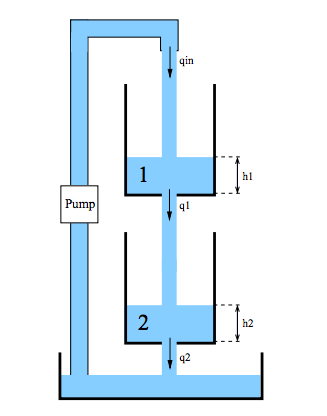
\includegraphics[width=70mm]{System.png}
\caption{Visualisering av labuppkopplingen}
\label{overflow}
\end{figure}

Pumpens reglersystem består av en spänningsregulator, mätsensorer för vattennivå samt programvara för PC baserad på LabView.
\newpage

% ------------- Resultat -----------------------
% Inte kommit längre än såhär /hanel742

\section{Resultat}

% ----- T ---

\subsection{Konstanten T}
Mätningen utfördes 3 gånger med samma steg från samma arbetspunkt. Resultatet av mätningarna ges i tabell 1 nedan. Arbetspunkten var under mätningarna 10cm (1,23V). Enhetssteget ökade nivån genom att spänningsnivån höjdes till 1,28V. 

\begin{table}[ht] 
\centering 
\begin{tabular}{c c} 
Försök & T \\ [0.5ex] % inserts table heading
\hline
1 & 17 \\
2 & 18 \\
3 & 20 \\

\end{tabular} 
\caption{Tabell över mätvärden på tidskonstanten.}

\end{table}
~\\ %weird ass quickfix
Medelvärdet på T räknades ut till T=18.4 och därmed var tidskonstanten bestämd. 
Bestämningen av K\textsubscript{dubbel} gick till på liknande vis. 

% ----- Kdubbel ---

\subsection{Konstanten K\textsubscript{dubbel}}

Mätningarna som utfördes för att söka K\textsubscript{dubbel} gjordes som sagt vid stationärt tillstånd. Dessa gjordes även de tre gånger men denna gång var steget lite olika från gång till gång. Resultatet av mätningarna ges i tabell 2 nedan. Arbetspunkten var under mätningarna 10cm (1,09V). Enhetssteget ökade nivån genom att spänningsnivån höjdes till 1,14V dvs med u=0,05V. 

\begin{table}[ht] 
\centering 
\begin{tabular}{c c} 
Försök & $\delta_{h2}$ \\ [0.5ex] % inserts table heading
\hline
1 & 1,46 \\
2 & 1,07 \\
3 & 1,36 \\

\end{tabular} 
\caption{Tabell över mätvärden på $\delta_{h2}$.}
\end{table}
~\\ %weird ass quickfix
Medelvärdet räknades ut till $\delta_{h2}=1,3$ vilket dividerat på u=0,05V ger K\textsubscript{dubbel}=25,9
\newpage
% ----- Fleadlag ---

\subsection{Förändring av systemets egenskaper}

Vi beräknade först ett reglersystem med hjälp av de givna specifikationerna, metoderna i Glad och Ljung (2006), samt vårt matlabscript. 
\\
\\
Systemet hade parametrarna K = 0,43, \textbeta = 0.2, \texttau{\textsubscript{D}} = 8,40, {\textsubscript{I}} = 37,60 och \textgamma = 0,465. Vi fick då ett system som reglerade enligt figur nedan. 

\begin{figure}[ht!]
\centering
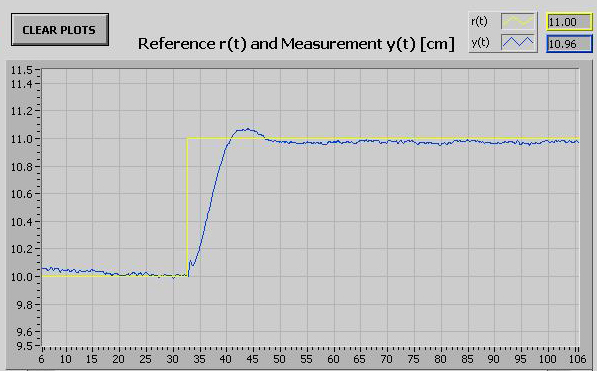
\includegraphics[width=90mm]{Test1_cut.jpg}
\caption{Stegsvaret efter kompensering med F\textsubscript{lead} och F\textsubscript{lag}.}
\label{overflow}
\end{figure}
~\\
Som synes presterar systemet väldigt nära specifikationerna - men stigtiden möter tyvärr inte riktigt kraven. Vi försökte då justera systemets stigtid till 4 sekunder. Tyvärr resulterade detta i en för stor översläng för systemet. Vi justerade då även ner kravet på översläng till 7\% istället för 10\%. Vi fick då en reglering som motsvarade specifikationen väl, se bild nedan. 

\begin{figure}[ht!]
\centering
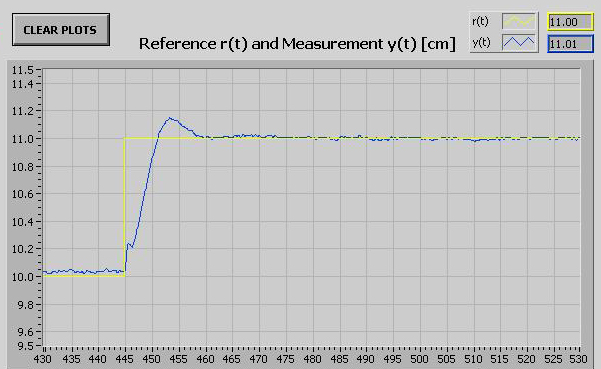
\includegraphics[width=90mm]{Test2_cut.jpg}
\caption{Stegsvaret efter kompensering med F\textsubscript{lead} och F\textsubscript{lag}.}
\label{overflow}
\end{figure}
~\\

Systemet körs med parametrarna K = 0,43, \textbeta = 0.2, \texttau{\textsubscript{D}} = 8,40, {\textsubscript{I}} = 37,60 och \textgamma = 0,465. 

% --------------------------------- Slutsats -------------------------

\newpage
\section{Slutsats}
Resultatet visar att Faskompensering med Flead och Flag fungerar alldeles utmärkt. Ett problem med metoden är dock att alla parametrar är mer eller mindre beroende av varandra. Under laboration utfördes därför finjustering av kurvan med att gå tillbaka och ändra någon grundparameter (exempelvis överslängsparametern M) för sedan köra om skriptet och producera nya variabler utifrån ändringen.
\\
\newline
Mätningarna av konstanterna K\textsubscript{enkel} och K\textsubscript{dubbel} utfördes endast tre gånger, för att kunna bestämma konstanterna mer exakt krävs mer mätvärden. Dessutom var det svårt att hålla en konstant arbetspunkt på 10 cm så steget utfördes inte alltid från exakt 10,00 cm. Detta kan bidra till ytterligare mätfel.


\newpage

% --------------------------------- Källor -------------------------

\section{Källor}
Glad, Torkel och Ljung, Lennart. 2006. \textit{Reglerteknik - Grundläggande teori}. Upplaga 4:10. Lund. Studentlitteratur AB.
\newpage

% --------------------------------- Appendix -------------------------

\section{Appendix A}
Matlabkod för beräkning av F\textsubscript{lead} och F\textsubscript{lag}.
\lstinputlisting{lab2_tankreglering.m}

\end{document}